% =====================================================================
% chapters/05_results.tex
% Chapter 5 — Results
% Project: Vision-Based Running Technique Classification from In-the-Wild
%          Internet Videos using Markerless Pose Estimation and Deep Learning
% =====================================================================

\chapter{Results}
\label{ch:results}

This chapter reports the empirical results of the running-technique
classification pipelines. Following the experimental protocol of
Chapter~\ref{ch:experimental-setup}, a strict separation is maintained
between (i)~\emph{controlled benchmark} results, obtained under the fixed
split-by-video protocol with a unified reporting procedure, and
(ii)~\emph{historical development} results, retained only as method-evolution
evidence. All controlled tables use the same fixed train/validation/test
split summarised in Section~\ref{sec:dataset-stats}. A separate fair-gap
robustness check then repeats the handmade--autocorr comparison under
5-fold video-level cross-validation to assess whether the fixed-split gap is
systematic.

% ---------------------------------------------------------------------
\section{Dataset Statistics}
\label{sec:dataset-stats}
% Source file: outputs/dataset/split_summary.csv

The dataset is partitioned by video identifier so that all cycles extracted
from a given video are confined to a single split, preventing video-specific
information from leaking between training and evaluation. Table~\ref{tab:split}
summarises the resulting split.

\begin{table}[htbp]
\centering
\caption[Dataset split by video and by detected running cycle. Source: \protect\path{split_summary.csv}.]{Dataset split by video and by detected running cycle. Source: \path{split_summary.csv}.}
\label{tab:split}
\tablefont
\begin{tabularx}{\textwidth}{X r r r r}
\toprule
\textbf{Split} & \textbf{Videos} & \textbf{Correct videos} & \textbf{False videos} & \textbf{Detected cycles} \\
\midrule
Train       & 52 & 20 & 32 & 97  \\
Validation  & 11 &  5 &  6 & 33  \\
Test        & 12 &  5 &  7 & 22  \\
\midrule
\textbf{Total} & \textbf{75} & \textbf{30} & \textbf{45} & \textbf{152} \\
\bottomrule
\end{tabularx}
\end{table}

The class balance at the video level is moderately skewed
toward the \emph{false} class (45 vs.\ 30), a distribution that motivates the
use of macro-averaged F1 as the primary evaluation metric throughout this
chapter, since macro-F1 weights both classes equally and is therefore
robust to this imbalance \cite{sokolova2009metrics}. The small validation and test
splits (11 and 12 videos respectively) also caution against over-interpreting
single-point differences, a consideration revisited in the discussion of
threshold tuning (Section~\ref{sec:threshold}).

% ---------------------------------------------------------------------
\section{Handmade Landmark Upper Bound}
\label{sec:handmade}
% Source file: outputs/handmade/handmade_results.csv

The handmade landmark pipeline uses manually controlled cycle segmentation and
therefore estimates the upper bound of the landmark representation under clean
cycle boundaries. It is not treated as a deployment baseline. Table~\ref{tab:handmade}
reports the four trained architectures.

\begin{table}[htbp]
\centering
\caption[Handmade landmark upper-bound results. Best macro-F1 and metrics in bold. Source: \protect\path{handmade_results.csv}.]{Handmade landmark upper-bound results. Best macro-F1 and metrics in bold. Source: \path{handmade_results.csv}.}
\label{tab:handmade}
\tablefont
\begin{tabularx}{\textwidth}{X r r r r r}
\toprule
\textbf{Model} & \textbf{Test acc.} & \textbf{Macro-F1} & \textbf{F1-correct} & \textbf{F1-false} & \textbf{ROC-AUC} \\
\midrule
MLP        & 0.8571 & 0.8545 & 0.8293 & 0.8798 & 0.9444 \\
1D-CNN     & 0.8929 & 0.8772 & 0.8889 & 0.8649 & 0.9444 \\
BiLSTM     & 0.8750 & 0.8623 & 0.8889 & 0.8357 & 0.9556 \\
\textbf{CNN-BiLSTM} & \textbf{0.9107} & \textbf{0.8991} & \textbf{0.9333} & \textbf{0.8649} & \textbf{0.9556} \\
\bottomrule
\end{tabularx}
\end{table}

The handmade setting establishes that the landmark representation is
learnable when cycle segmentation is reliable, with all four architectures
exceeding 0.85 macro-F1 and ROC-AUC above 0.94. This directly answers the first research
question: when running cycles are correctly segmented, the markerless pose
representation carries sufficient information for a deep model to discriminate
correct from false technique. The narrow spread across
architectures (macro-F1 0.8545--0.8991) indicates that, given clean cycles,
classification is not strongly architecture-limited.

% ---------------------------------------------------------------------
\section{Autocorr Landmark Baseline}
\label{sec:autocorr-baseline}
% Source files: outputs/autocorr/autocorr_results.csv,
%               outputs/autocorr/autocorr_cycle_stats.csv

The autocorrelation landmark pipeline is the main automatic baseline. It uses
the \texttt{contact\_diff} motion signal, autocorrelation period estimation,
foot-strike-to-foot-strike cycle cutting, no cycle margin, selected landmark
features, and velocity features. Table~\ref{tab:autocorr} reports the
controlled fixed-split results.

\begin{table}[htbp]
\centering
\caption[Autocorr landmark baseline results. Best macro-F1 in bold. Source: \protect\path{autocorr_results.csv}.]{Autocorr landmark baseline results. Best macro-F1 in bold. Source: \path{autocorr_results.csv}.}
\label{tab:autocorr}
\small
\begin{tabular}{lrrrrr}
\toprule
Model & Test acc. & Macro-F1 & F1-correct & F1-false & ROC-AUC \\
\midrule
MLP & 0.5455 & 0.5417 & 0.5000 & 0.5833 & 0.6068 \\
1D-CNN & 0.5000 & 0.3425 & 0.6850 & 0.0000 & 0.5684 \\
BiLSTM & 0.4545 & 0.3714 & 0.7429 & 0.0000 & 0.5342 \\
CNN-BiLSTM & \textbf{0.5909} & \textbf{0.5901} & 0.5333 & 0.6468 & \textbf{0.6370} \\
\bottomrule
\end{tabular}
\end{table}

% SỬA LỖI DÒNG 149 TẠI ĐÂY: Thay \sec:threshold} bằng \ref{sec:threshold}
Although the CNN-BiLSTM has the best fixed-threshold macro-F1 in the raw
autocorr model table, the thesis baseline uses the MLP row in later summary
tables because the threshold analysis in Section~\ref{sec:threshold} shows it
is more stable after validation-based threshold selection. This distinction is
important: the automatic baseline is evaluated not only by its peak
fixed-threshold score but also by its robustness to the complete reporting
protocol. Compared with the handmade upper bound, the autocorr landmark baseline drops
substantially. The best fixed-threshold automatic result reaches only 0.5901
macro-F1, and the robust reported MLP baseline reaches 0.5417 macro-F1. Some
sequential models collapse on the \emph{false} class so dominantly that F1-false reaches 0.0000.
This validation-to-test collapse, combined with ROC-AUC values close to 0.5,
indicates that the limiting factor in the automatic pipeline is not classifier
capacity but the quality and consistency of the automatically segmented
cycles. The contrast with Section~\ref{sec:handmade} is quantified directly in Section~\ref{sec:hm-vs-ac}.

\IfFileExists{figures/autocorr_confusion_matrix.png}{%
\begin{figure}[htbp]
\centering
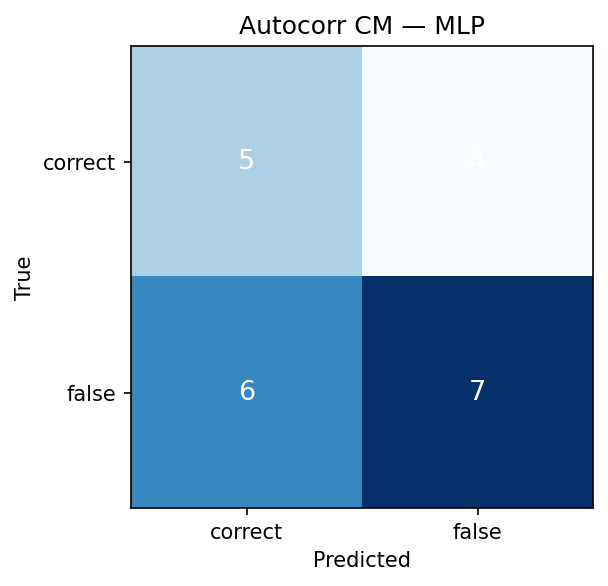
\includegraphics[width=0.65\textwidth]{figures/autocorr_confusion_matrix.png}
\caption[Confusion matrix for autocorr-based landmark pipeline on test split.]{Confusion matrix for the autocorrelation-based landmark pipeline on the controlled test split.}
\label{fig:autocorr-confusion-matrix}
\end{figure}
}{}

% ---------------------------------------------------------------------
\section{Handmade versus Autocorr Comparison}
\label{sec:hm-vs-ac}
% Source file: figures/main_pipeline_comparison.csv

Table~\ref{tab:hm-ac} gives the main controlled comparison between clean
manual cycles and automatic autocorrelation cycles. The rows use the same
landmark representation family, so the comparison isolates the effect of cycle
source.

\begin{table}[htbp]
\centering
\caption[Main comparison between handmade upper bound and autocorr baseline. Source: \protect\path{main_pipeline_comparison.csv}.]{Main comparison between handmade upper bound and autocorr automatic landmark baseline. Best controlled result in bold. Source: \path{main_pipeline_comparison.csv}.}
\label{tab:hm-ac}
\small
% Sử dụng tabularx với cột X đầu tiên giúp tự động xuống dòng các tên Pipeline quá dài
\begin{tabularx}{\textwidth}{X l r r r r r}
\toprule
\textbf{Pipeline} & \textbf{Cycle source} & \textbf{Test acc.} & \textbf{Macro-F1} & \textbf{F1-correct} & \textbf{F1-false} & \textbf{ROC-AUC} \\
\midrule
Handmade landmark upper bound & Manual & \textbf{0.9107} & \textbf{0.8991} & \textbf{0.9333} & \textbf{0.8649} & \textbf{0.9556} \\
\addlinespace
Autocorr landmark baseline & Automatic & 0.5455 & 0.5417 & 0.5000 & 0.5833 & 0.6068 \\
\bottomrule
\end{tabularx}
\end{table}

Replacing handmade cycles with automatic cycles reduces accuracy by
0.3652 (from 0.9107 to 0.5455) and macro-F1 by 0.3574 (from 0.8991 to 0.5417).
Because both pipelines share the same landmark representation, classifier
family, split, and reporting protocol, this gap is attributable primarily to
the cycle-segmentation stage rather than to the classifier. This is the
central empirical finding of the thesis: the markerless representation is
\emph{learnable} (Section~\ref{sec:handmade}) but the automatic
\emph{segmentation} of in-the-wild running cycles is the dominant bottleneck.
The detection-stage statistics also show why: the
\texttt{contact\_diff} pipeline retains only 151 of its raw cycles and fails
to detect usable cycles in a substantial number of videos
(Section~\ref{sec:signal-ablation}). Section~\ref{sec:fair-gap} tests the
same interpretation under repeated video-level folds.

\begin{figure}[htbp]
\centering
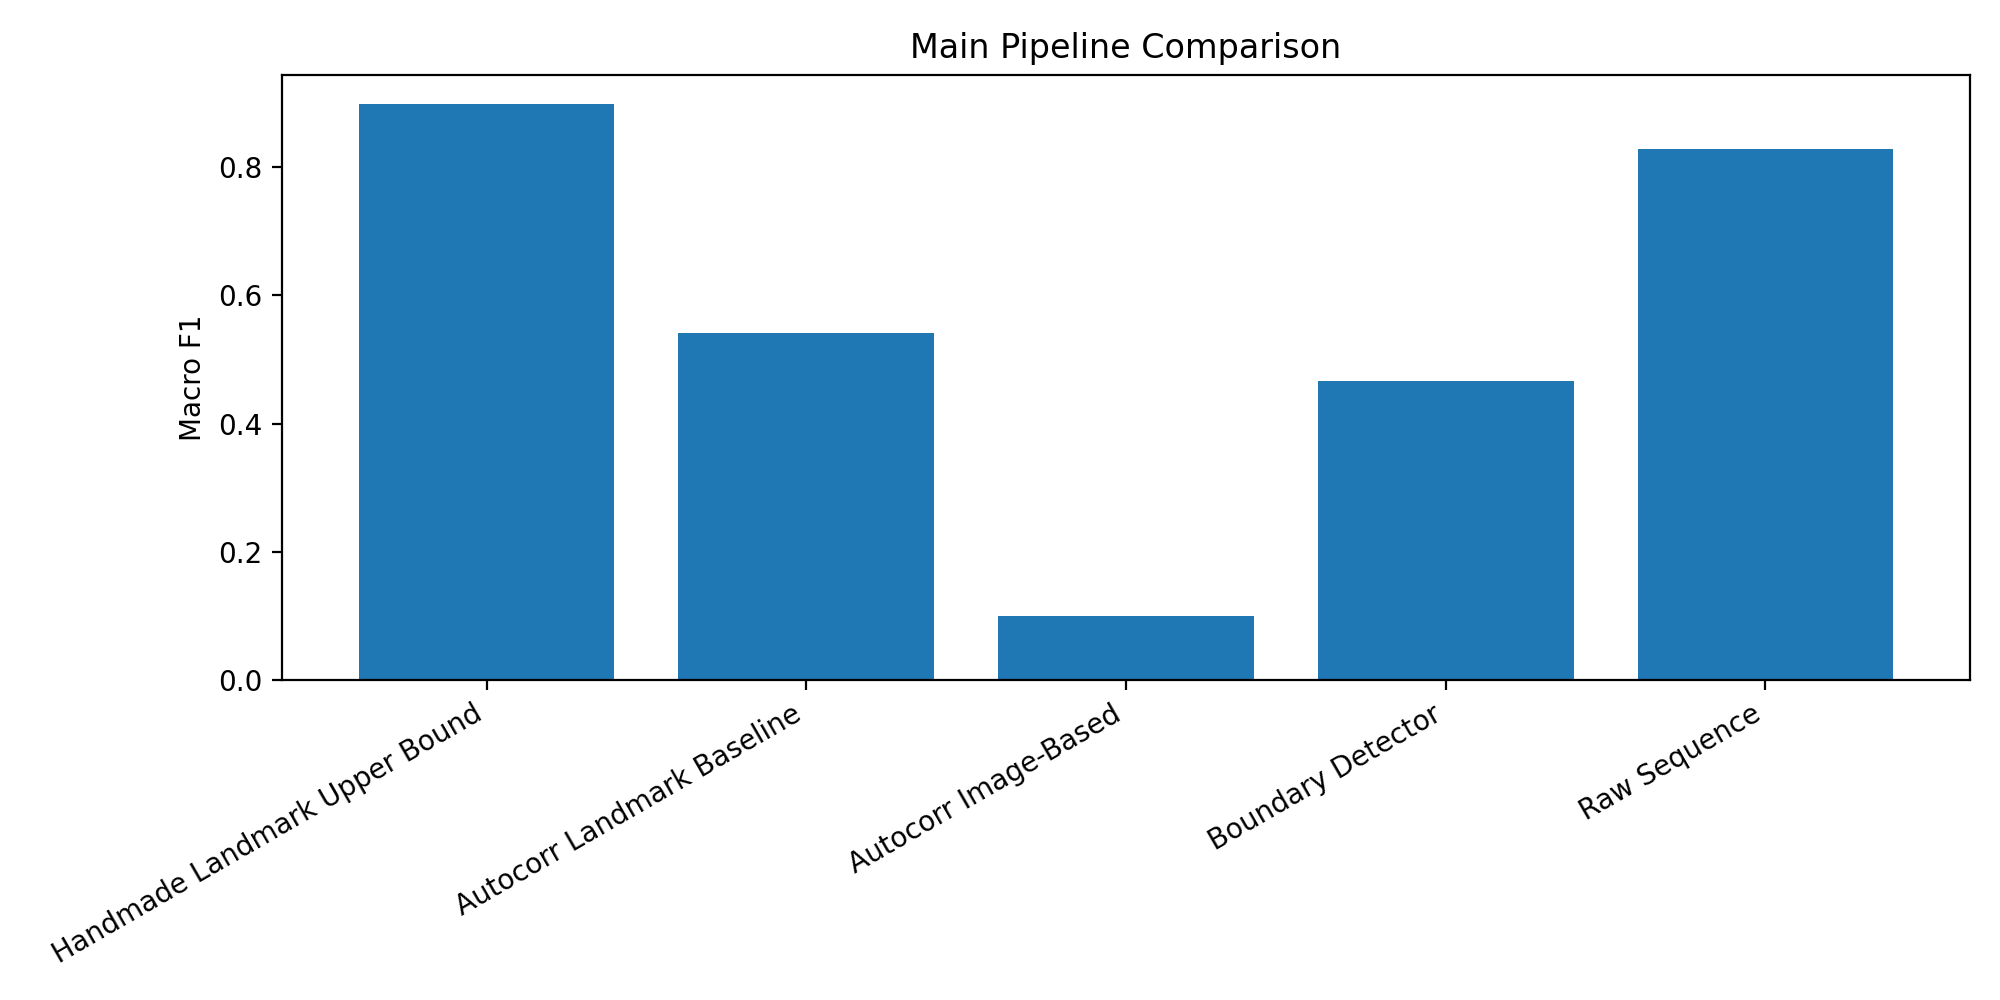
\includegraphics[width=0.85\textwidth]{figures/main_pipeline_comparison.png}
\caption[Main pipeline comparison. Source: \protect\path{main_pipeline_comparison.png}.]{Main pipeline comparison between the handmade landmark upper bound, the autocorr landmark baseline, and supplementary pipelines. Source: \path{main_pipeline_comparison.png}.}
\label{fig:main-pipeline-comparison}
\end{figure}


% ---------------------------------------------------------------------
\section{Fair Gap Robustness Check}
\label{sec:fair-gap}

The fixed-split comparison in Section~\ref{sec:hm-vs-ac} gives the primary
controlled benchmark, but the validation and test sets are small. To test
whether the handmade--autocorr gap was merely a difficult split artefact, an
additional fair-gap robustness check was conducted. Both cycle sources were
evaluated using the same MLP classifier, 5-fold video-level cross-validation,
a fixed threshold of $0.5$, and macro-F1 as the main metric.

\begin{table}[htbp]
\centering
\caption[Fair-gap robustness check under 5-fold video-level CV. Source: \protect\path{fair_gap_and_mlp_perm.csv}.]{Fair-gap robustness check under 5-fold video-level cross-validation using the same MLP classifier and threshold $0.5$. Source: \path{outputs/autocorr/fair_gap_and_mlp_perm.csv}.}
\label{tab:fair-gap-cv}
\small
\begin{tabularx}{\textwidth}{X r r r l}
\toprule
\textbf{Cycle source} & \textbf{Cycles} & \textbf{Videos} & \textbf{CV macro-F1} & \textbf{OOF macro-F1, 95\% CI} \\
\midrule
Handmade cycles & 370 & 369 & $0.860 \pm 0.016$ & $0.860$ [0.822, 0.897] \\
Autocorr cycles & 151 & 55  & $0.615 \pm 0.081$ & $0.655$ [0.580, 0.728] \\
\midrule
\multicolumn{3}{l}{\textbf{Fair gap (handmade $-$ autocorr)}} & \textbf{0.245} & -- \\
\bottomrule
\end{tabularx}
\end{table}

Table~\ref{tab:fair-gap-cv} confirms the same conclusion as the fixed-split
benchmark. Handmade cycles remain stable under repeated video-level folds,
achieving $0.860 \pm 0.016$ macro-F1. Autocorr cycles remain substantially
weaker, achieving $0.615 \pm 0.081$ macro-F1. The resulting fair gap of 0.245
macro-F1 is smaller than the single fixed-split gap of 0.3574, but it remains
large enough to show that the performance loss is systematic rather than only
the result of one difficult split.

A permutation test was then applied to the autocorr MLP setting to assess
whether the observed autocorr features were robustly separable under the same
simple classifier. With 100 random label permutations, the observed CV macro-F1
was 0.5206, while the null distribution had a mean of 0.468 and a standard
deviation of 0.074, giving $p = 0.2475$. This does not establish statistically
significant separation from the permutation baseline. The result should be read
conservatively: autocorr-derived cycles contain some discriminative signal, as
also reflected by the CV comparison, but the signal is noisy and not robustly
separable under the tested MLP configuration.

\begin{table}[htbp]
\centering
\caption[Permutation test for the autocorr MLP setting. Source: \protect\path{fair_gap_and_mlp_perm.json}.]{Permutation test for the autocorr MLP setting. Source: \path{outputs/autocorr/fair_gap_and_mlp_perm.json}.}
\label{tab:autocorr-permutation}
\small
\begin{tabularx}{\textwidth}{X r}
\toprule
\textbf{Quantity} & \textbf{Value} \\
\midrule
Observed autocorr CV macro-F1 & 0.5206 \\
Null mean macro-F1 & 0.4680 \\
Null standard deviation & 0.0740 \\
Number of permutations & 100 \\
Permutation $p$-value & 0.2475 \\
\bottomrule
\end{tabularx}
\end{table}


% ---------------------------------------------------------------------
\section{Model Ablation Results}
\label{sec:model-ablation}
% Source file: outputs/ablation/model_ablation.csv

The model ablation compares MLP, 1D-CNN, BiLSTM, and CNN-BiLSTM architectures
under the handmade and autocorr pipelines. Table~\ref{tab:model-ablation}
shows the macro-F1 and accuracy for each setting.

\begin{table}[htbp]
\centering
\caption[Model ablation on handmade and autocorr pipelines. Source: \protect\path{model_ablation.csv}.]{Model ablation on handmade and autocorr pipelines. Best macro-F1 within each pipeline in bold. Source: \path{model_ablation.csv}.}
\label{tab:model-ablation}
\small
\begin{tabular}{llrrr}
\toprule
Pipeline & Model & Test acc. & Macro-F1 & ROC-AUC \\
\midrule
\multirow{4}{*}{Handmade}
& MLP & 0.8571 & 0.8545 & 0.9444 \\
& 1D-CNN & 0.8929 & 0.8772 & 0.9444 \\
& BiLSTM & 0.8750 & 0.8623 & \textbf{0.9556} \\
& CNN-BiLSTM & \textbf{0.9107} & \textbf{0.8991} & \textbf{0.9556} \\
\midrule
\multirow{4}{*}{Autocorr}
& MLP & 0.5455 & 0.5417 & 0.6068 \\
& 1D-CNN & 0.5000 & 0.3425 & 0.5684 \\
& BiLSTM & 0.4545 & 0.3714 & 0.5342 \\
& CNN-BiLSTM & \textbf{0.5909} & \textbf{0.5901} & \textbf{0.6370} \\
\bottomrule
\end{tabular}
\end{table}

The architecture effect is pipeline-dependent. In the handmade setting, the
hybrid CNN-BiLSTM performs best, suggesting that local pose patterns and
temporal ordering are both useful when the eight phases are correctly aligned.
In the automatic setting, model ranking becomes unstable: at a 0.5 threshold the CNN-BiLSTM is best (macro-F1 0.5901), whereas the
simpler MLP wins once thresholds are tuned (Section~\ref{sec:threshold}). The
absolute values remain low for every automatic-pipeline model, reinforcing
that architecture choice cannot recover the information lost to imperfect
segmentation.

% ---------------------------------------------------------------------
\section{Feature Ablation Results}
\label{sec:feature-ablation}
% Source file: outputs/ablation/feature_ablation.csv

The feature ablation fixes the classifier and varies only the input feature
set, on the handmade pipeline. Table~\ref{tab:feature-ablation} reports the
resulting performance.

\begin{table}[htbp]
\centering
\caption[Feature ablation on handmade cycles. Source: \protect\path{feature_ablation.csv}.]{Feature ablation on handmade cycles. Best macro-F1 in bold. Source: \path{feature_ablation.csv}.}
\label{tab:feature-ablation}
\small
\begin{tabular}{lrrrr}
\toprule
Feature set & Test acc. & Macro-F1 & F1-false & ROC-AUC \\
\midrule
Selected 13 landmarks & 0.9107 & \textbf{0.8991} & 0.8649 & \textbf{0.9556} \\
All 33 landmarks & 0.8929 & 0.8961 & \textbf{0.9189} & 0.9389 \\
Lower-body only & 0.8929 & 0.8961 & \textbf{0.9189} & 0.9222 \\
Selected 13 + velocity & 0.9107 & \textbf{0.8991} & 0.8649 & \textbf{0.9556} \\
\bottomrule
\end{tabular}
\end{table}

The selected 13-landmark representation matches the best macro-F1 while
remaining lower-dimensional than the full 33-landmark representation. The
lower-body-only and all-landmark variants improve F1-false but do not improve
macro-F1 overall, suggesting that additional coordinates can alter class
balance without yielding a more robust classifier. The selected-landmark
configurations cluster tightly around 0.90~macro-F1, supporting the use of the
compact 13-landmark representation as the pipeline default for the automatic
experiments, where added input dimensionality offers little benefit relative
to its sensitivity to landmark noise.

% ---------------------------------------------------------------------
\section{Signal Ablation Results}
\label{sec:signal-ablation}
% Source file: outputs/ablation/signal_ablation.csv

The signal ablation compares the seven candidate motion signals used for
cycle detection, holding the classifier family fixed. Table~\ref{tab:signal}
reports detection coverage and classification performance.

\begin{table}[htbp]
\centering
\caption[Cycle-detection signal ablation. Source: \protect\path{signal_ablation.csv}.]{Cycle-detection signal ablation. Best macro-F1 and best retained cycle count are bolded separately. Source: \path{signal_ablation.csv}.}
\label{tab:signal}
\small
\begin{tabular}{lrrrrr}
\toprule
Signal & Test acc. & Macro-F1 & Videos OK & Cycles retained & Cycles rejected \\
\midrule
head\_y & 0.6818 & 0.6703 & \textbf{72} & \textbf{204} & 13 \\
hip\_y & \textbf{0.7333} & \textbf{0.7321} & 67 & 190 & 15 \\
heel\_y & 0.6667 & 0.6623 & 35 & 49 & 36 \\
toe\_y & 0.5000 & 0.5000 & 35 & 52 & 33 \\
contact\_diff & 0.5909 & 0.5901 & 50 & 151 & 42 \\
AP\_diff & 0.2500 & 0.2000 & 32 & 33 & 39 \\
V\_diff & 0.6364 & 0.6022 & 48 & 125 & 34 \\
\bottomrule
\end{tabular}
\end{table}

The \texttt{hip\_y} signal achieves the highest classification macro-F1 in this
ablation, while \texttt{contact\_diff} is retained as the main baseline signal
because it reflects foot-contact dynamics and produces more semantically
aligned cycle boundaries. The decision is not based on accuracy alone. In this
thesis, the baseline signal must support foot-strike-to-foot-strike sampling,
eight-phase interpretation, and stable comparison to the image pipeline. The
\texttt{contact\_diff} signal therefore produces the most temporally coherent
foot-strike-to-foot-strike boundaries, consistent with periodic gait-cycle structure in human motion \cite{cutting1978gaitperiodicity,plotnik2007gaitasymmetry}, which is why it is adopted as the
baseline cycle-detection signal even though its classification macro-F1
(0.5901) is not the single highest. The vertical signals
(\texttt{head\_y}, \texttt{hip\_y}) detect more videos but admit many
ill-formed cycles, illustrating the trade-off between detection coverage and
boundary precision that underlies the segmentation bottleneck identified in
Section~\ref{sec:hm-vs-ac}.

% ---------------------------------------------------------------------
\section{Frames-per-Cycle Ablation Results}
\label{sec:frames-ablation}
% Source file: outputs/ablation/frames_ablation.csv

The frame ablation tests whether increasing temporal resolution beyond the
eight-phase representation improves performance on handmade cycles. Table~\ref{tab:frames} summarises the best model at each frame count.

\begin{table}[htbp]
\centering
\caption[Frames-per-cycle ablation on handmade cycles. Source: \protect\path{frames_ablation.csv}.]{Frames-per-cycle ablation on handmade cycles. Best macro-F1 in bold. Source: \path{frames_ablation.csv}.}
\label{tab:frames}
\small
\begin{tabular}{lrrrr}
\toprule
Frames per cycle & Best model & Test acc. & Macro-F1 & ROC-AUC \\
\midrule
8 & CNN-BiLSTM & 0.9107 & \textbf{0.8991} & \textbf{0.9556} \\
16 & BiLSTM & 0.8750 & 0.8623 & \textbf{0.9556} \\
24 & CNN-BiLSTM & 0.8393 & 0.8347 & 0.9389 \\
32 & CNN-BiLSTM & 0.8571 & 0.8545 & 0.9444 \\
\bottomrule
\end{tabular}
\end{table}

The eight-phase representation gives the best macro-F1 despite being the
shortest sequence. Sixteen frames remain highly competitive
(BiLSTM macro-F1 0.8623 at the lowest cost), and increasing frame count
yields no monotonic improvement. This supports the eight-phase sampling
choice as an efficient representation of the running cycle, with additional
temporal resolution providing diminishing returns on this dataset.

% ---------------------------------------------------------------------
\section{Autocorr Version History and Method Evolution}
\label{sec:version-history}
% Source file: figures/autocorr_version_comparison.csv

This section documents the evolution of the autocorrelation pipeline. The
values in Table~\ref{tab:version-history} are \emph{historical} validation
figures drawn from development notebooks; they are presented as method-evolution
evidence only and must not be read as controlled benchmark results. Where a
metric was never recorded under the controlled protocol it is marked
\texttt{[MISSING RESULT]}.

\begin{table}[htbp]
\centering
\caption[Autocorr version history and development evidence.]{Autocorr version history (historical development evidence --- not a controlled benchmark). Source: \protect\path{autocorr_version_comparison.csv}.}
\label{tab:version-history}
\footnotesize
\begin{tabularx}{\textwidth}{l X l X r}
\toprule
\textbf{Version} & \textbf{Signal} & \textbf{Input} & \textbf{Model} & \textbf{Val. acc. (\%)} \\
\midrule
\texttt{autocorr\_fixed\_val\_acc\_69\_6} & head-Y oscillation & landmarks & CNN+LSTM & 69.6 \\
\addlinespace
% SỬA LỖI DÒNG 161+ TẠI ĐÂY: Thêm dấu escape \% ở 69.6\%, 72.9\%, 76.5\% để không bị lỗi Missing $
\texttt{autocorr\_fixed\_val\_acc\_72\_9} & \texttt{contact\_diff} & landmarks & CNN+LSTM & 72.9 \\
\addlinespace
\texttt{autocorr\_fixed\_biLSTM} & \texttt{contact\_diff} & landmarks $+$ vel. & BiLSTM & 65.0 \\
\addlinespace
\texttt{autocorr\_fixed\_val\_acc\_76\_5} & \texttt{contact\_diff} & RGB crop $224^2$ & MobileNetV2$+$LSTM & 76.5 \\
\midrule
\texttt{02\_baseline\_landmark} & \texttt{contact\_diff} & 13 lm $+$ vel. & best of 4 & \multicolumn{1}{c}{$^{\dagger}$} \\
\bottomrule
\end{tabularx}
\end{table}

\begin{figure}[htbp]
\centering
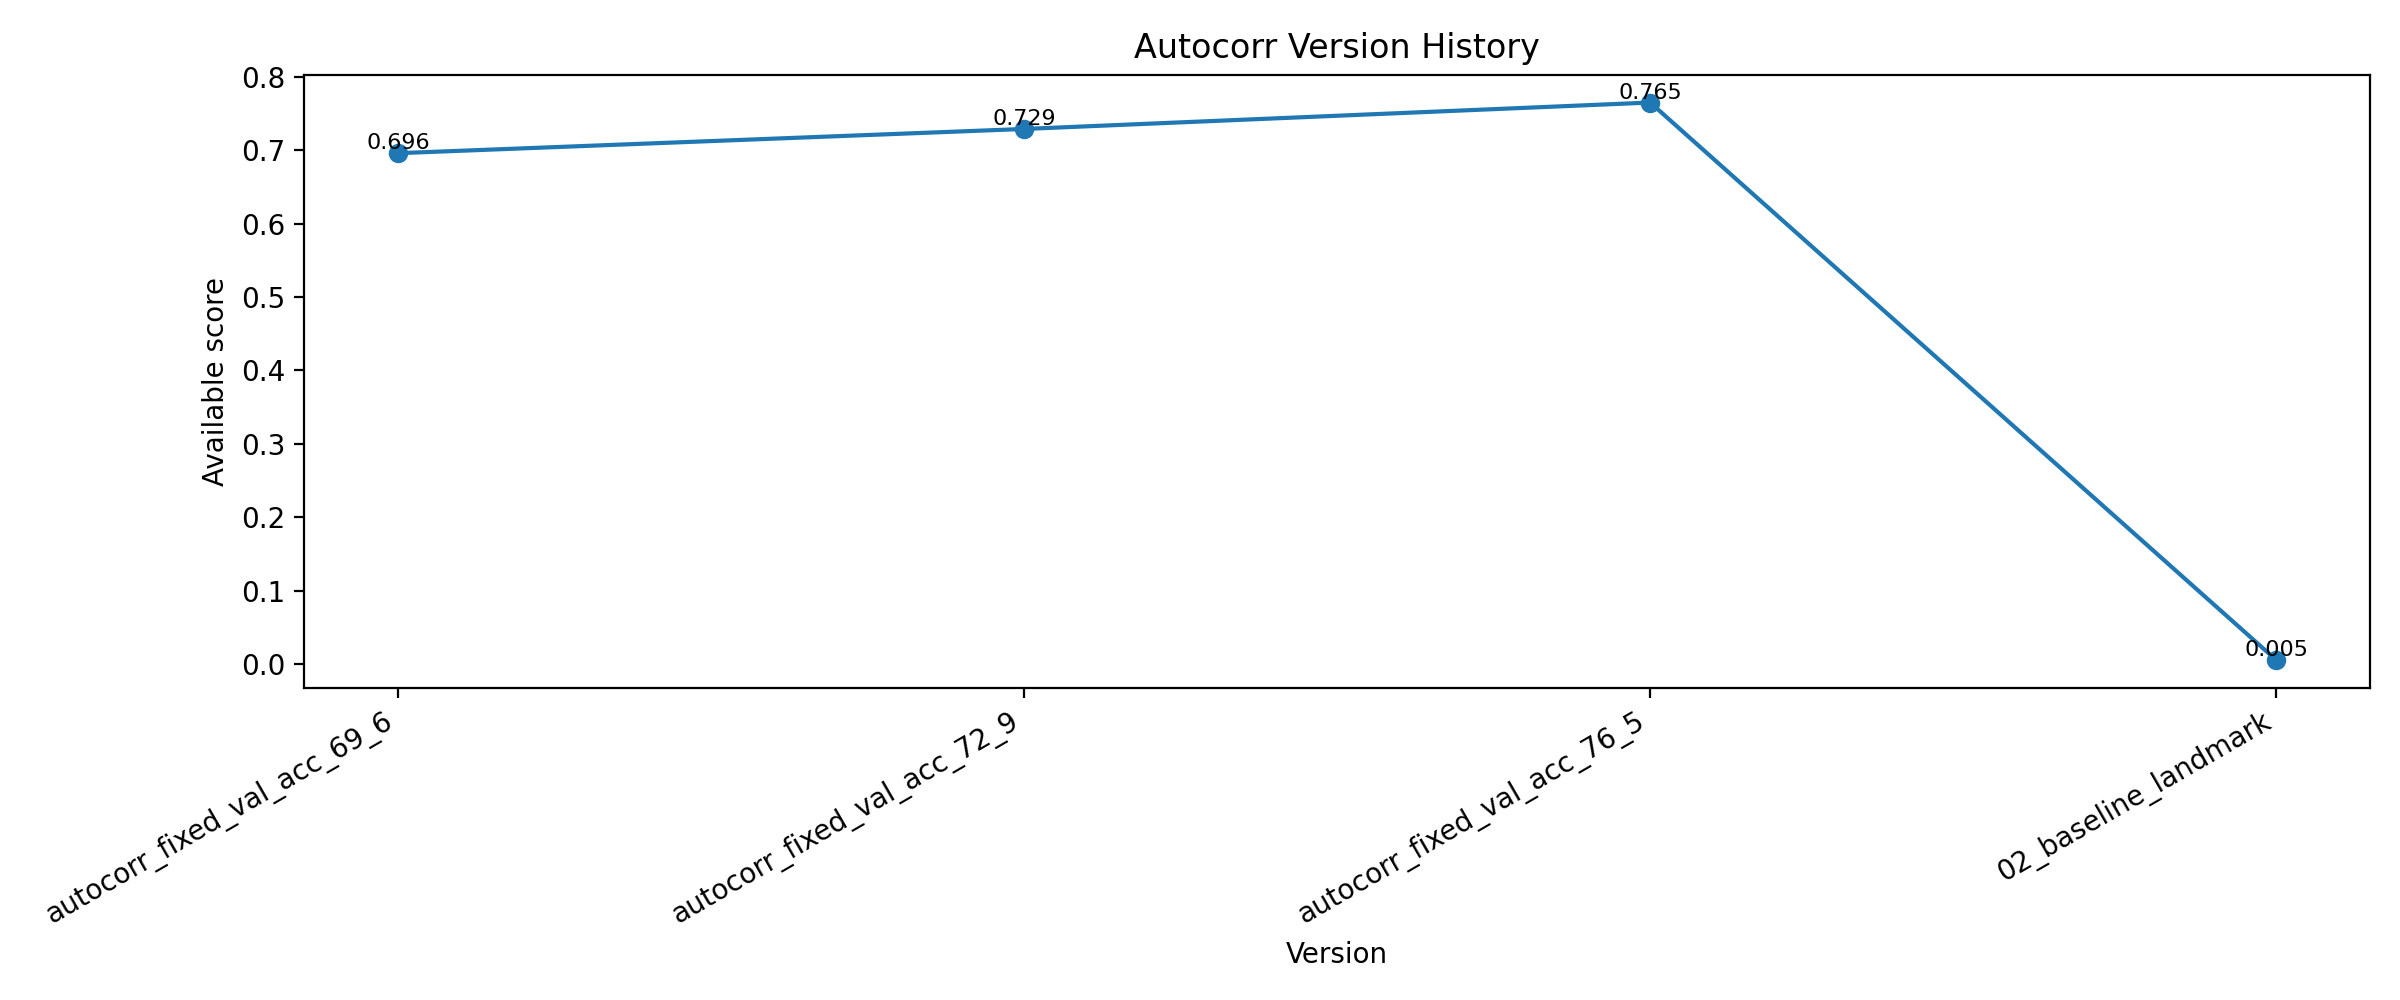
\includegraphics[width=0.85\textwidth]{figures/autocorr_version_history.png}
\caption[Historical autocorr method evolution.]{Historical autocorr method evolution. This figure is development evidence only; Source: \path{autocorr_version_history.png}.}
\label{fig:autocorr-version-history}
\end{figure}

\noindent$^{\dagger}$ The \texttt{02\_baseline\_landmark} row is the only
controlled entry; under the fixed-split protocol it records a test accuracy of
0.5455 and a test macro-F1 of 0.5417 (Section~\ref{sec:autocorr-baseline}), in
[0,1] rather than percent. Its historical validation accuracy was not recorded
(\texttt{[MISSING RESULT]}).

The development trace shows three substantive changes: replacing the noisy
head-Y oscillation signal with \texttt{contact\_diff} (historical validation
69.6\% $\rightarrow$ 72.9\%), adopting autocorrelation period estimation with
foot-strike-to-foot-strike alignment, and an exploratory shift to an
image-based representation (\texttt{autocorr\_fixed\_val\_acc\_76\_5}). The
76.5\% figure is the most technically complex historical milestone, but it is
a development validation accuracy on an RGB-crop representation and was not
re-confirmed under the controlled protocol; it is therefore retained as
motivation for the organised image-based rerun
(Section~\ref{sec:image-results}) rather than as evidence that image-based
modelling outperforms the landmark baseline.

% ---------------------------------------------------------------------
\section{Autocorr Image-Based Results}
\label{sec:image-results}
% Source file: outputs/autocorr_image/image_results.csv

The image-based pipeline is the \emph{controlled} rerun of the historical
image idea: it reuses the exact \texttt{contact\_diff}/autocorrelation cycle
source of the landmark baseline, but represents each phase as a runner-centred
RGB crop processed by a MobileNetV2$+$LSTM model \cite{sandler2018mobilenetv2,hochreiter1997lstm,donahue2015lrcn}. Table~\ref{tab:image}
reports the controlled result.

\begin{table}[htbp]
\centering
\caption[Autocorr image-based pipeline results. Source: \protect\path{image_results.csv}.]{Autocorr image-based pipeline (controlled rerun). Source: \path{image_results.csv}.}
\label{tab:image}
\small
\begin{tabular}{llrrrr}
\toprule
Input & Model & Test acc. & Macro-F1 & F1-false & ROC-AUC \\
\midrule
RGB crop & MobileNetV2$+$LSTM & 0.1111 & 0.1000 & 0.2000 & 0.0592 \\
\bottomrule
\end{tabular}
\end{table}

Under the controlled protocol the image-based pipeline reaches a test macro-F1
of only 0.1000, with F1-correct of 0.0000 and a ROC-AUC of 0.0592, i.e.\ far
below chance. The model effectively fails to learn a usable decision boundary
on this small dataset. Crucially, this controlled result does \emph{not}
reproduce the historical 76.5\% validation figure of
Section~\ref{sec:version-history}, which underscores why that figure cannot
serve as a benchmark. The collapse is consistent with the known fragilities of
the image representation on limited in-the-wild data: bounding-box and crop
instability, domain shift, and overfitting of a high-capacity visual backbone \cite{sandler2018mobilenetv2}.
This indicates that the current image-based implementation
is not yet stable enough to replace the landmark baseline, not that image-based
modelling is invalid in principle.

\IfFileExists{figures/image_confusion_matrix.png}{%
\begin{figure}[htbp]
\centering
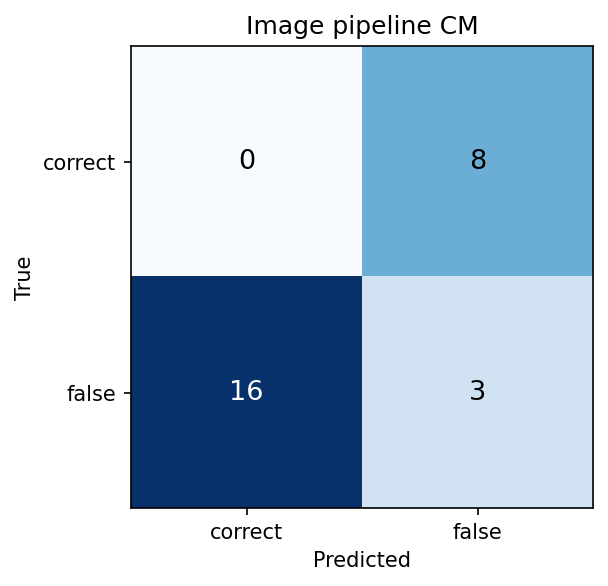
\includegraphics[width=0.65\textwidth]{figures/image_confusion_matrix.png}
\caption[Confusion matrix for the image-based pipeline.]{Confusion matrix for the image-based pipeline on the controlled test split.}
\label{fig:image-confusion-matrix}
\end{figure}
}{}

% ---------------------------------------------------------------------
\section{Landmark-Based versus Image-Based Representation}
\label{sec:representation}
% Source file: figures/representation_comparison.csv
%              (video-level: representation_video_level_comparison.csv)

Table~\ref{tab:repr} compares the two representations on the same automatic
cycle source, at the cycle (sample) level.

\begin{table}[htbp]
\centering
\caption[Landmark vs image representation. Source: \protect\path{representation_comparison.csv}.]{Landmark versus image representation (controlled), identical cycle source. Source: \path{representation_comparison.csv}.}
\label{tab:repr}
\small
\begin{tabular}{llrrrr}
\toprule
Representation & Model & Test acc. & Macro-F1 & ROC-AUC & Test samples \\
\midrule
Landmark & MLP & \textbf{0.5455} & \textbf{0.5417} & 0.6068 & 22 \\
Image & MobileNetV2$+$LSTM & 0.1111 & 0.1000 & 0.0592 & 27 \\
\bottomrule
\end{tabular}
\end{table}

On a matched cycle source, the landmark representation clearly outperforms the
image representation (macro-F1 0.5417 versus 0.1000).The same ordering holds at the video level, where the landmark pipeline reaches 0.6250 accuracy / 0.6190 macro-F1 under majority voting against 0.2857 / 0.2222 for the image pipeline (\path{representation_video_level_comparison.csv}).
For this dataset and
implementation, the sparse landmark sequence is the more reliable
representation; the RGB-crop pipeline does not add usable discriminative
information and is markedly less stable. This addresses the
representation research question while remaining within the controlled
protocol, separately from the historical 76.5\% milestone.

\begin{figure}[htbp]
\centering
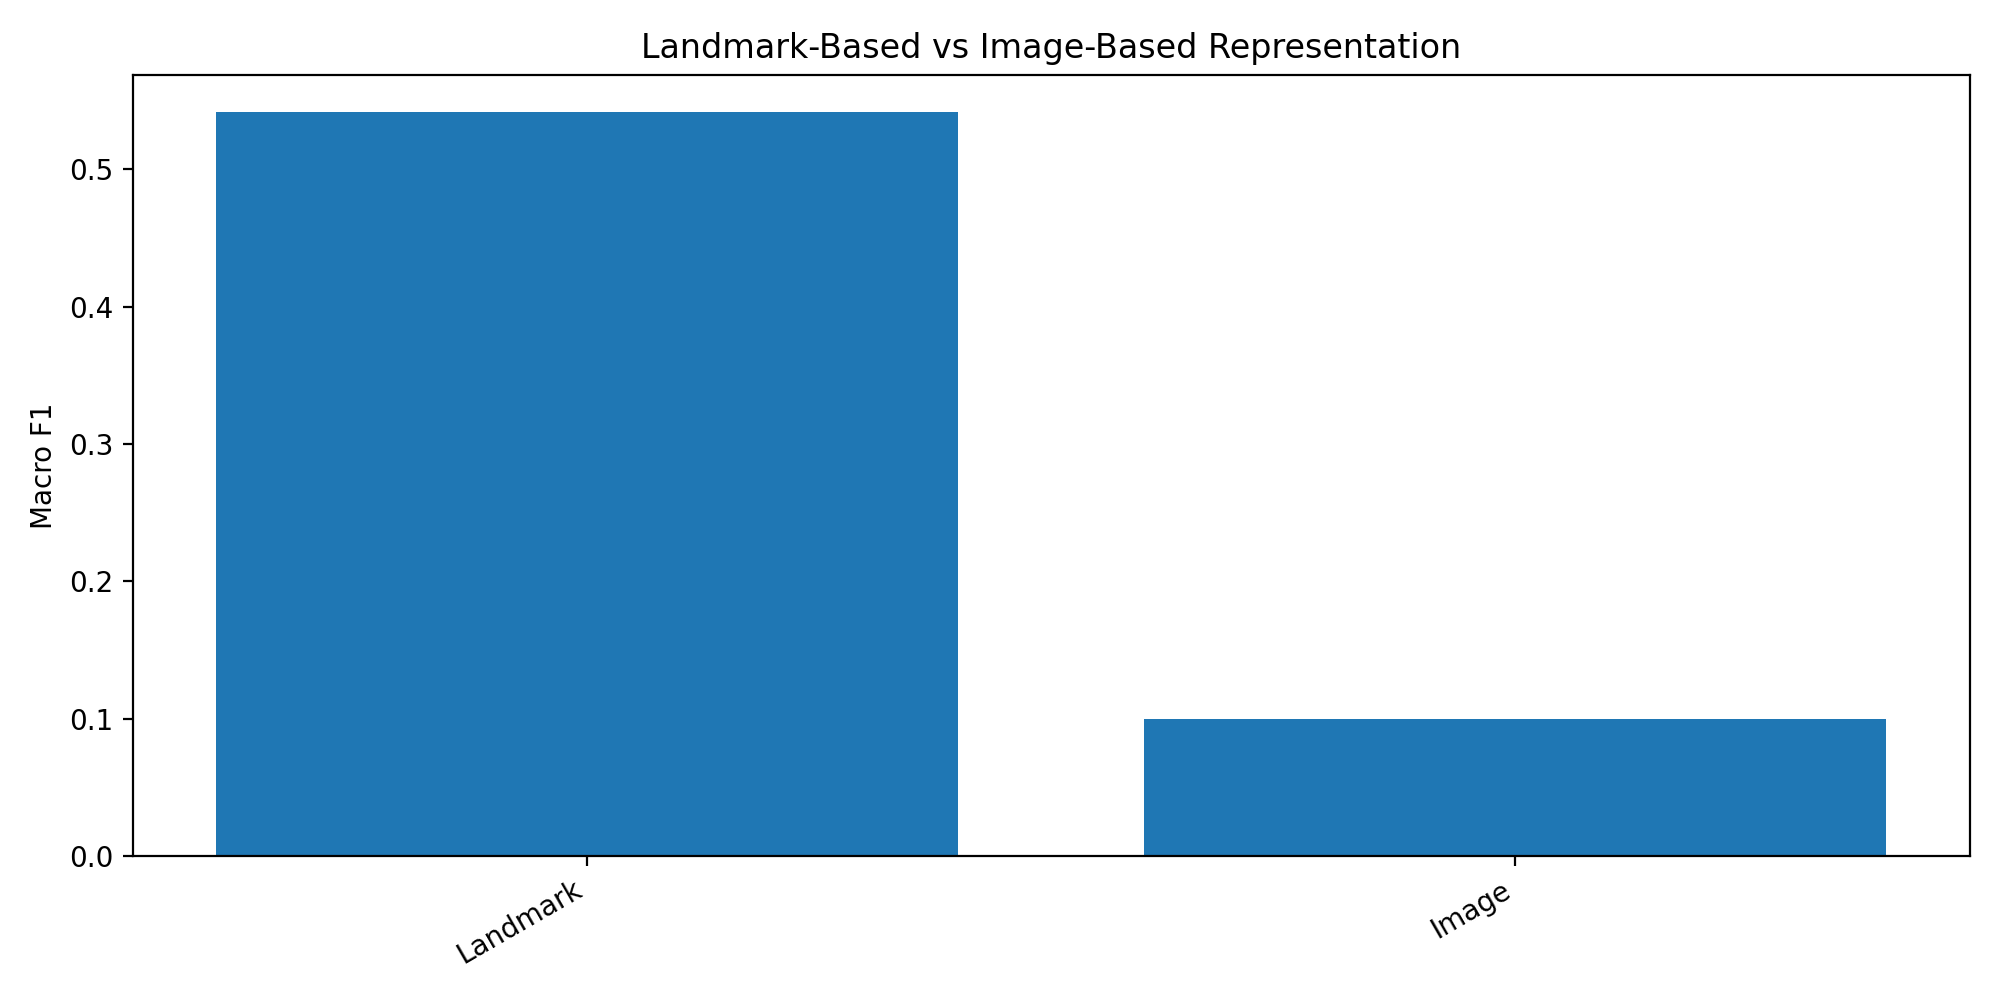
\includegraphics[width=0.85\textwidth]{figures/landmark_vs_image_comparison.png}
\caption[Controlled landmark-versus-image comparison.]{Controlled landmark-versus-image representation comparison under the automatic autocorr cycle source. Source: \path{landmark_vs_image_comparison.png}.}
\label{fig:landmark-vs-image-comparison}
\end{figure}

% ---------------------------------------------------------------------
\section{Cycle-Level versus Video-Level Evaluation}
\label{sec:cycle-vs-video}
% Source files: figures/cycle_level_metrics.csv,
%               figures/video_level_metrics.csv

Because each video may yield several cycles, predictions can be reported per
cycle or aggregated per video. Table~\ref{tab:cyc-vid} compares the two for the
automatic landmark baseline (the main pipeline) and lists the supplementary
pipelines for reference.

\begin{table}[htbp]
\centering
\caption[Cycle-level versus video-level evaluation.]{Cycle-level versus video-level evaluation. Video-level uses majority vote. Sources: \protect\path{cycle_level_metrics.csv}, \protect\path{video_level_metrics.csv}.}
\label{tab:cyc-vid}
\small
\begin{tabular}{llrrrr}
\toprule
Pipeline & Level & Acc. & Macro-F1 & F1-false & $N$ \\
\midrule
\multirow{2}{*}{Autocorr (baseline)}
& Cycle & 0.5238 & 0.5139 & 0.5833 & 21 \\
& Video (majority) & \textbf{0.5714} & \textbf{0.5333} & 0.6667 & 7 \\
\midrule
Image & Cycle & 0.1111 & 0.1000 & 0.2000 & 27 \\
Image & Video (majority) & 0.2857 & 0.2222 & 0.4444 & 7 \\
\midrule
Boundary Detector & Cycle & 0.6000 & 0.5833 & 0.5000 & 5 \\
Boundary Detector & Video (majority) & 0.6667 & 0.6667 & 0.6667 & 3 \\
\midrule
Raw sequence & Cycle/Video & 0.8182 & 0.8036 & 0.8571 & 11 \\
\bottomrule
\end{tabular}
\end{table}

For the automatic landmark baseline, aggregating cycle predictions to the video
level by majority vote improves both accuracy (0.5238 $\rightarrow$ 0.5714) and
macro-F1 (0.5139 $\rightarrow$ 0.5333). The same direction appears for the image
and boundary-detector pipelines. This indicates that per-cycle predictions
contain noise that partially cancels under aggregation, so video-level reporting
gives a fairer estimate of practical performance. The very
small video counts ($N=3$--$7$) mean these gains, while consistent in
direction, rest on few samples and should be treated as indicative.

\begin{figure}[htbp]
\centering
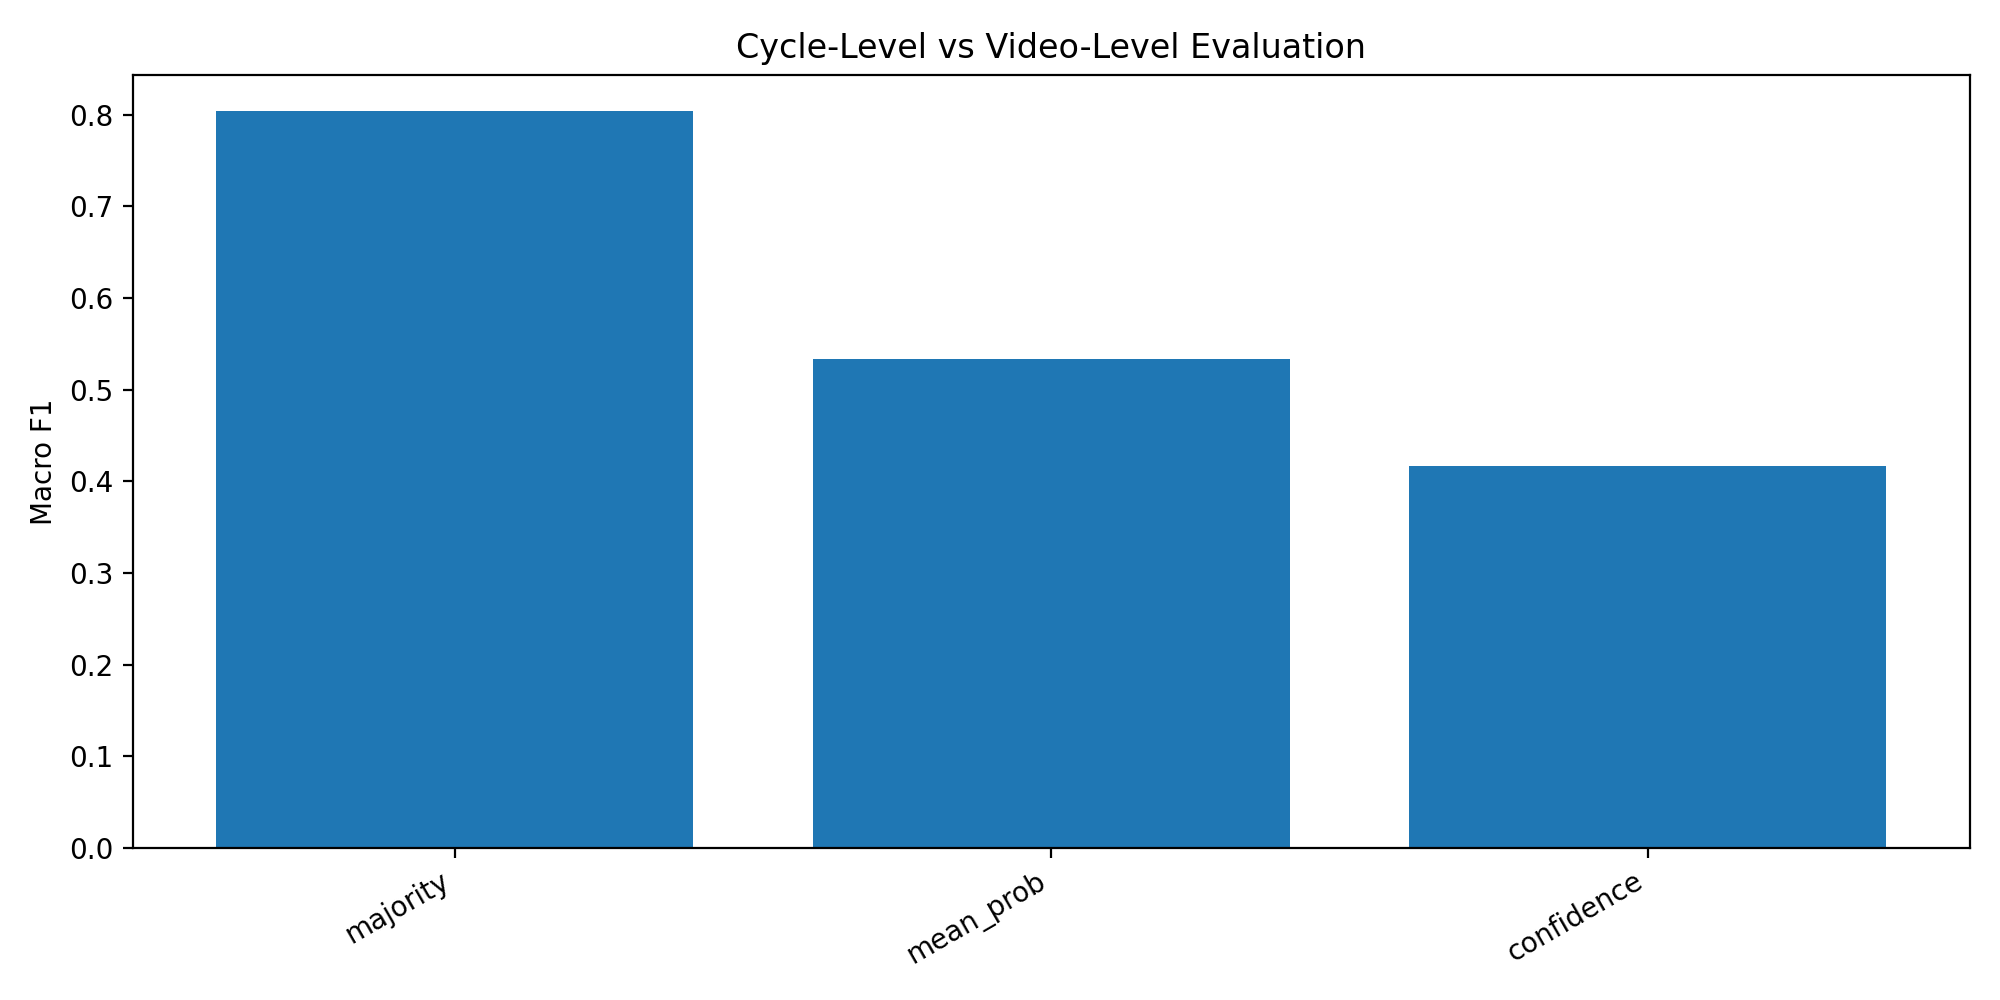
\includegraphics[width=0.85\textwidth]{figures/cycle_vs_video_comparison.png}
\caption[Cycle-level versus video-level evaluation.]{Cycle-level versus video-level evaluation. Video-level predictions aggregate cycle predictions by majority voting. Source: \path{cycle_vs_video_comparison.png}.}
\label{fig:cycle-vs-video-comparison}
\end{figure}

% ---------------------------------------------------------------------
\section{Threshold 0.5 versus Tuned Threshold}
\label{sec:threshold}
% Source file: figures/threshold_05_vs_tuned.csv

Decision thresholds tuned on validation can either improve or overfit test
performance. Table~\ref{tab:threshold} reports, for each model, the macro-F1 at
the default 0.5 threshold and at the validation-selected threshold, together
with the change and an overfit flag.

\begin{table}[htbp]
\centering
\caption[Default threshold versus validation-tuned threshold.]{Default threshold versus validation-tuned threshold. Thresholds are selected on validation and applied to test. Source: \protect\path{threshold_05_vs_tuned.csv}.}
\label{tab:threshold}
\tablefont
\begin{adjustbox}{max width=\textwidth}
\begin{tabular}{llrrrrl}
\toprule
Pipeline & Model & Macro-F1@0.5 & Best thr. & Tuned macro-F1 & $\Delta$ & Overfit \\
\midrule
\multirow{4}{*}{Handmade}
& 1D-CNN & 0.8961 & 0.34 & 0.8772 & $-0.0189$ & True \\
& BiLSTM & 0.8772 & 0.78 & 0.8772 & $0.0000$ & False \\
& CNN-BiLSTM & 0.8772 & 0.40 & \textbf{0.8991} & $+0.0219$ & False \\
& MLP & 0.8250 & 0.16 & 0.8545 & $+0.0295$ & False \\
\midrule
\multirow{4}{*}{Autocorr}
& MLP & 0.5417 & 0.34 & \textbf{0.5417} & $0.0000$ & False \\
& 1D-CNN & 0.3425 & 0.50 & 0.3425 & $0.0000$ & False \\
& BiLSTM & 0.3714 & 0.54 & 0.2903 & $-0.0811$ & True \\
& CNN-BiLSTM & 0.5901 & 0.18 & 0.4359 & $-0.1542$ & True \\
\midrule
Image & all & 0.1000 & \texttt{[MISSING RESULT]} & \texttt{[MISSING RESULT]} & \texttt{[MISSING RESULT]} & False \\
\bottomrule
\end{tabular}
\end{adjustbox}
\end{table}

On the clean handmade pipeline, validation-tuned thresholds mostly help or are
neutral (CNN-BiLSTM improves to 0.8991). On the automatic pipeline the picture
reverses: tuning leaves the MLP unchanged but severely degrades the sequential
models, with the CNN-BiLSTM dropping by 0.1542 macro-F1 and being flagged as
threshold-overfit. This explains the apparent disagreement with the model
ablation (Section~\ref{sec:model-ablation}): the CNN-BiLSTM is best at the 0.5
threshold but unstable once a validation-selected threshold is applied, whereas
the MLP is the robust choice for the reported baseline. The
image pipeline exposes only an aggregate row with no probability-based sweep, so
its tuned entries are \texttt{[MISSING RESULT]}. All reported baseline metrics
state explicitly whether a 0.5 or tuned threshold was used.

\begin{figure}[htbp]
\centering
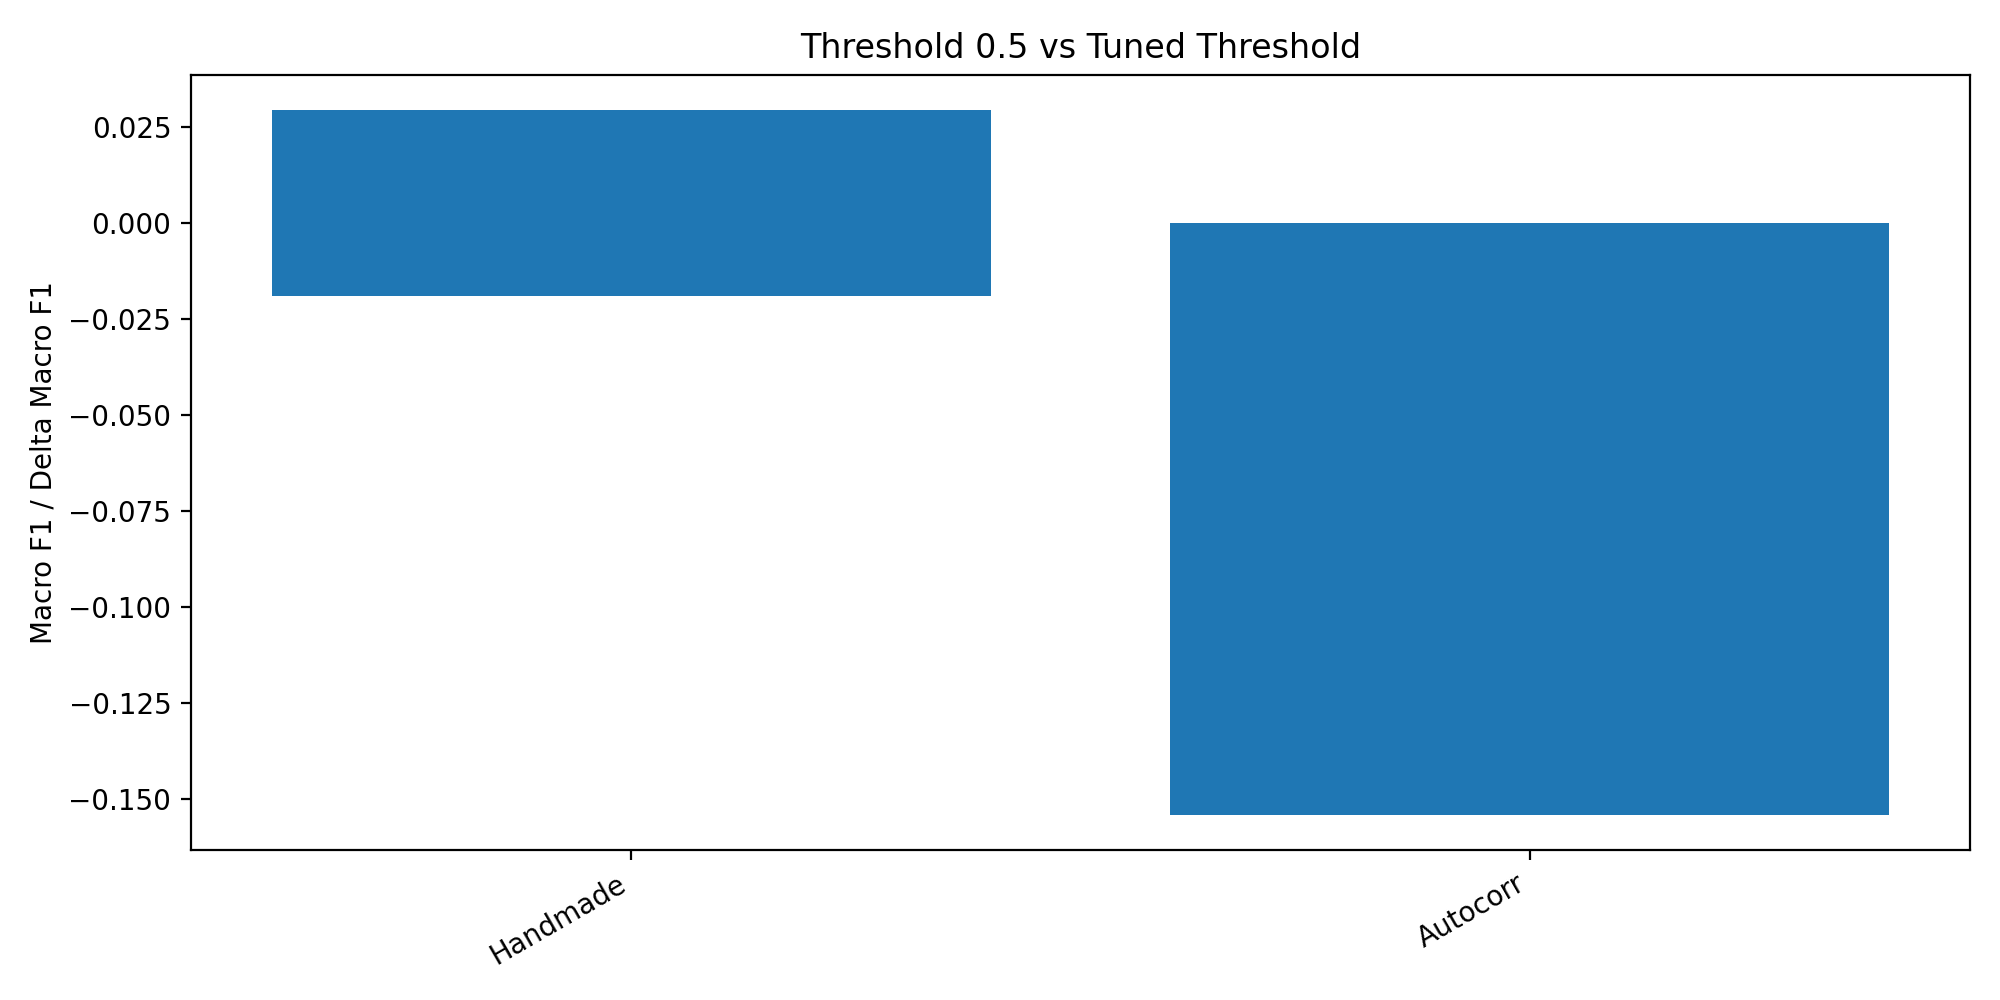
\includegraphics[width=0.85\textwidth]{figures/threshold_comparison.png}
\caption[Comparison between default 0.5 threshold and tuned thresholds.]{Comparison between the default 0.5 decision threshold and validation-tuned thresholds. Source: \path{threshold_comparison.png}.}
\label{fig:threshold-comparison}
\end{figure}

% ---------------------------------------------------------------------
\section{Pose and Cycle Quality Analysis}
\label{sec:quality}
% Source file: figures/pose_cycle_quality_metrics.csv

To locate the source of automatic-pipeline errors, test cycles are grouped by
pose- and cycle-quality factors (median split) and accuracy/macro-F1 compared
across groups. Table~\ref{tab:quality} reports representative factors; within
each factor the higher-accuracy group is bold.

\begin{table}[htbp]
\centering
\caption[Pose and cycle quality analysis (Autocorr baseline).]{Pose and cycle quality analysis (Autocorr baseline). Median-split groups. Source: \protect\path{pose_cycle_quality_metrics.csv}.}
\label{tab:quality}
\small
\begin{tabular}{llrrr}
\toprule
Quality factor & Group & $n$ & Acc. & Macro-F1 \\
\midrule
\multirow{2}{*}{Heel visibility}
& low ($\le 0.91$) & 11 & 0.4545 & 0.4107 \\
& high ($>0.91$) & 11 & \textbf{0.6364} & 0.5417 \\
\midrule
\multirow{2}{*}{Autocorr correlation}
& low ($\le 0.59$) & 18 & 0.5000 & 0.4582 \\
& high ($>0.59$) & 4 & \textbf{0.7500} & 0.4286 \\
\midrule
\multirow{2}{*}{Missing-ratio proxy}
& low ($\le 0.05$) & 11 & \textbf{0.6364} & 0.5417 \\
& high ($>0.05$) & 11 & 0.4545 & 0.4107 \\
\midrule
\multirow{2}{*}{Cycle duration}
& low ($\le 0.88$) & 16 & 0.5000 & 0.4921 \\
& high ($>0.88$) & 6 & \textbf{0.6667} & \textbf{0.6667} \\
\midrule
\multirow{2}{*}{Cycle period}
& low ($\le 0.77$) & 12 & \textbf{0.5833} & 0.5556 \\
& high ($>0.77$) & 10 & 0.5000 & 0.3333 \\
\bottomrule
\end{tabular}
\end{table}

The accuracy trends are consistent with the segmentation-bottleneck
interpretation: cycles with higher heel visibility (0.6364 vs.\ 0.4545), lower
landmark missing-ratio (0.6364 vs.\ 0.4545), and stronger autocorrelation
(0.7500 vs.\ 0.5000) are classified more accurately. In other words, errors
concentrate where pose estimation is unreliable or the periodic signal is weak,
rather than being uniformly distributed. Several
high-quality groups are very small ($n=4$--$6$), so the magnitudes are
indicative; the direction, however, points clearly at upstream pose and cycle
quality as the dominant error source for the automatic pipeline. A complementary
breakdown of failed videos (\texttt{failed\_video\_quality\_summary.csv})
attributes the majority of failures to the cycle-detection stage.

\begin{figure}[htbp]
\centering
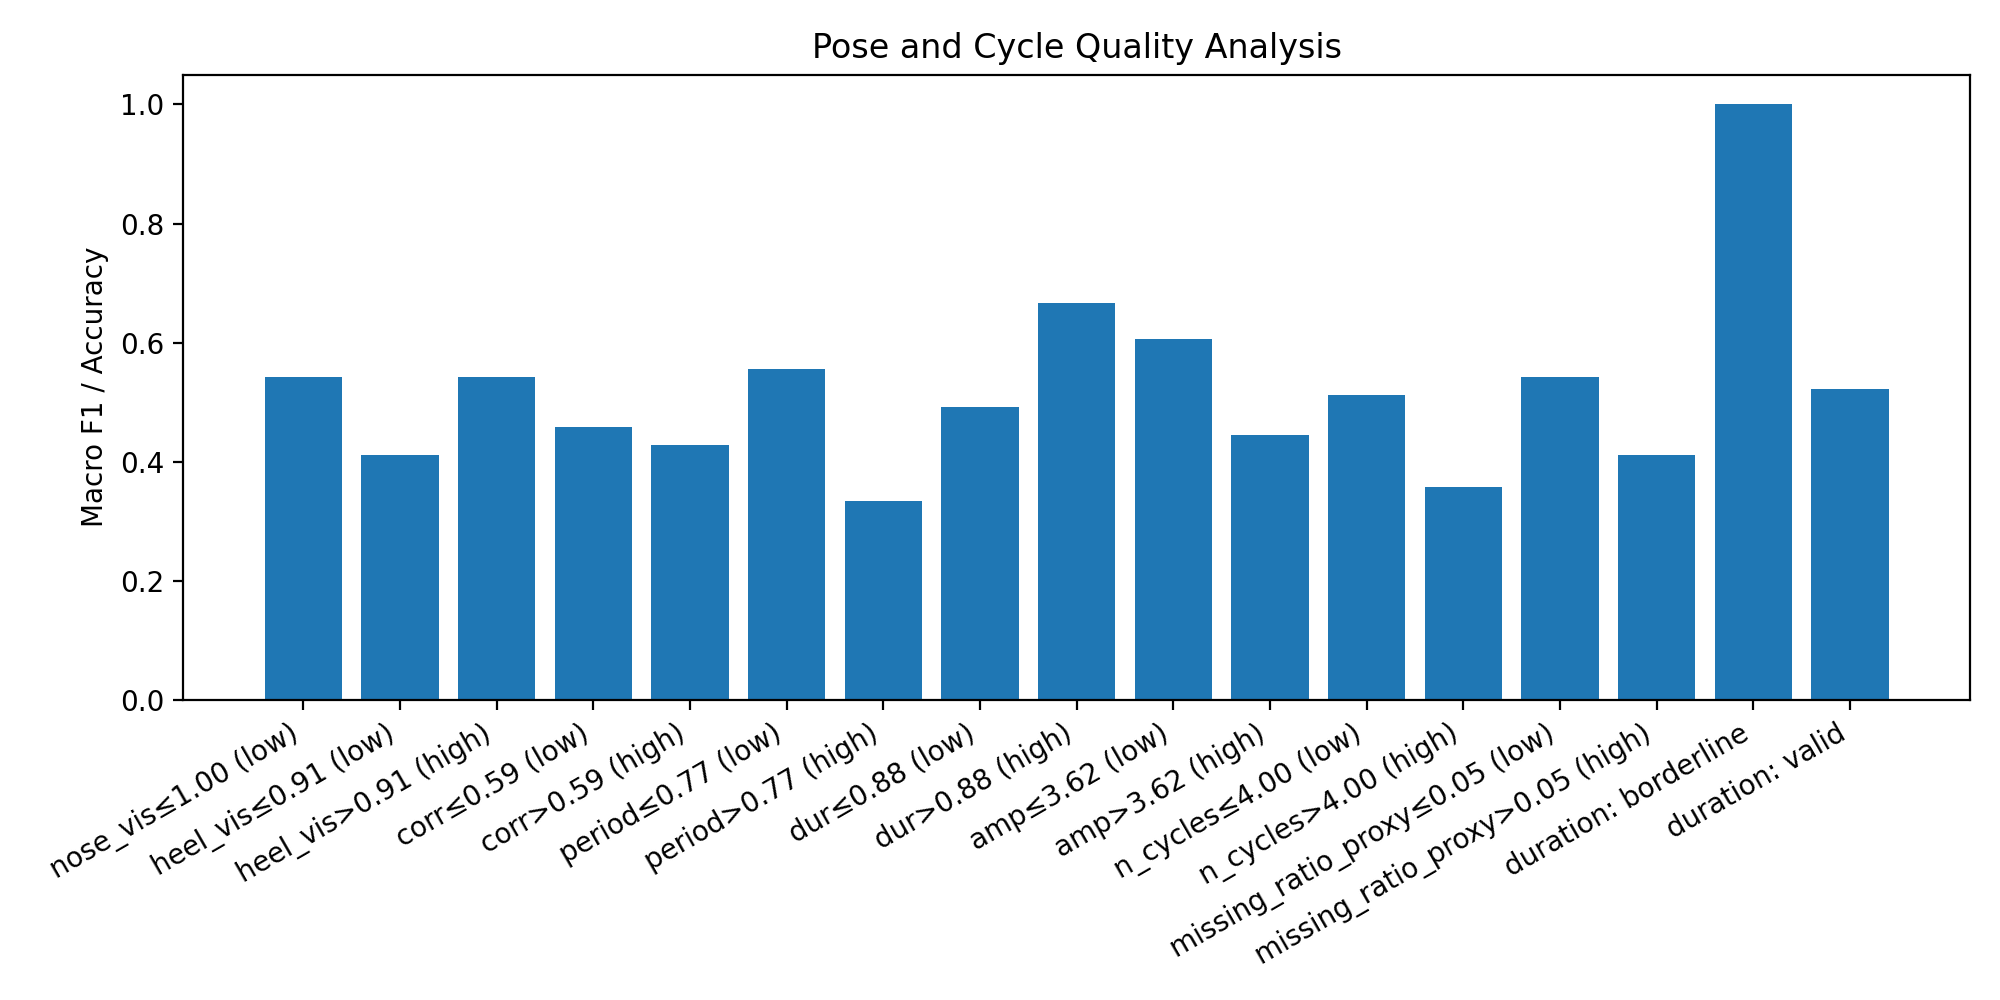
\includegraphics[width=0.85\textwidth]{figures/quality_analysis_summary.png}
\caption[Pose and cycle quality summary.]{Pose and cycle quality summary for the automatic landmark pipeline. Source: \path{quality_analysis_summary.png}.}
\label{fig:quality-analysis-summary}
\end{figure}

% ---------------------------------------------------------------------
\section{Boundary Detector and Raw Sequence Results}
\label{sec:bd-raw}

Two exploratory alternatives to rule-based cycle detection are reported here as
supplementary evidence. The learned Boundary Detector replaces autocorrelation
with a BiLSTM foot-strike detector; the raw-sequence model classifies the whole
pose sequence without explicit cycle cutting (one sample per video). Table~\ref{tab:bd-raw} summarises their best configurations.

\begin{table}[htbp]
\centering
\caption[Boundary Detector and raw-sequence pipelines.]{Boundary Detector and raw-sequence pipelines (Supplementary results). Sources: \protect\path{main_pipeline_comparison.csv}, \protect\path{bd_results.csv}, and \protect\path{raw_sequence_results.csv}.}
\label{tab:bd-raw}
\tablefont
\begin{adjustbox}{max width=\textwidth}
\begin{tabular}{llrrrr}
\toprule
Pipeline & Best config. & Test acc. & Macro-F1 & F1-false & ROC-AUC \\
\midrule
Boundary Detector & BiLSTM & 0.5000 & 0.4667 & 0.3333 & \texttt{[MISSING RESULT]} \\
Raw sequence & BiLSTM, seq$=16$, selected & 0.8333 & 0.8286 & 0.8571 & \texttt{[MISSING RESULT]} \\
\bottomrule
\end{tabular}
\end{adjustbox}
\end{table}

The Boundary Detector (best macro-F1 0.4667) does not improve on the
autocorrelation baseline and remains limited by the same scarce, noisy cycle
boundaries. The raw-sequence BiLSTM reports a high macro-F1 (0.8286), but this
figure is computed over only 12 video-level test samples and uses a different
evaluation unit (one sequence per video) than the cycle-level benchmarks; it
is therefore reported as an exploratory direction rather than as evidence that
cycle cutting is unnecessary. ROC-AUC was not stored for
either pipeline (\texttt{[MISSING RESULT]}). Both are kept out of the main
controlled comparison.

% ---------------------------------------------------------------------
\section{Summary of Main Findings}
\label{sec:summary}

Table~\ref{tab:summary} consolidates the controlled pipelines alongside the
supplementary ones. The best \emph{controlled benchmark} is bold. The
image-based row is shown without bold emphasis, in line with its exploratory
status, and the historical 76.5\% milestone of
Section~\ref{sec:version-history} is deliberately excluded from this benchmark
table.

\begin{table}[htbp]
\centering
\caption[Summary of pipeline results.]{Summary of pipeline results. The best controlled benchmark is bolded. Source: \protect\path{main_pipeline_comparison.csv}.}
\label{tab:summary}
\tablefont
\begin{adjustbox}{max width=\textwidth}
\begin{tabular}{lllrrrr}
\toprule
Pipeline & Input & Model & Acc. & Macro-F1 & F1-false & ROC-AUC \\
\midrule
\multicolumn{7}{l}{\emph{Controlled benchmark}} \\
Handmade upper bound & 13 lm $+$ vel. & CNN-BiLSTM & \textbf{0.9107} & \textbf{0.8991} & 0.8649 & 0.9556 \\
Autocorr landmark baseline & landmark feats. & MLP & 0.5455 & 0.5417 & 0.5833 & 0.6068 \\
Autocorr image-based & RGB crop & MobileNetV2$+$LSTM & 0.1111 & 0.1000 & 0.2000 & 0.0592 \\
\midrule
\multicolumn{7}{l}{\emph{Supplementary; small $N$, not controlled benchmark}} \\
Boundary Detector & landmark seq. & BiLSTM & 0.5000 & 0.4667 & 0.3333 & \texttt{[MISSING RESULT]} \\
Raw sequence & selected, seq$=16$ & BiLSTM & 0.8333 & 0.8286 & 0.8571 & \texttt{[MISSING RESULT]} \\
\bottomrule
\end{tabular}
\end{adjustbox}
\end{table}

The results give a coherent answer to the thesis research questions. First,
the markerless pose representation is sufficient to classify correct versus
false running technique when cycles are clean: the handmade upper bound reaches
0.8991 macro-F1. Second, automatic cycle detection is the dominant bottleneck:
the matched automatic baseline falls to 0.5417 macro-F1, a fixed-split gap of
0.3574. A separate 5-fold video-level CV check confirms that this is not only a
single-split artefact: handmade cycles reach $0.860 \pm 0.016$ macro-F1, while
autocorr cycles reach $0.615 \pm 0.081$, leaving a fair gap of 0.245. Together,
the ablations and robustness check attribute the loss to segmentation and pose
quality rather than to the classifier or temporal resolution. Third, within the controlled protocol
the compact landmark representation is more reliable than the RGB-crop image
representation, which collapses on this small dataset. The supplementary
boundary-detector and raw-sequence pipelines do not overturn these conclusions.
Taken together, the evidence supports investing future work in robust cycle
segmentation and pose quality rather than in larger classifiers or richer image
representations. Consistent with this scope, the results do
not claim real-world deployment readiness.